YouTube-8M\textsuperscript{\cite{abu2016youtube}} คือชุดข้อมูลวิดีโอที่มีจำนวนวิดีโอเยอะที่สุดถึง 8 ล้านวิดีโอ (พ.ศ. 2559) โดยมีจุดมุ่งหมายหลักในการจำแนกสาระสำคัญของวิดีโอ (video theme) 
ด้วยคำสั้นๆ เช่น ถ้าวิดีโอนั้นมีมนุษย์กำลังปั่นจักรยานบนถนนดินริมหน้าผาชุดข้อมูลนี้จะกำกับวิดีโอนี้ว่า mountain biking ซึ่งทำให้ YouTube-8M 
แตกต่างจากชุดข้อมูลวิดีโออื่นๆส่วนใหญ่ที่จะเน้นการกระทำหรือกิจกรรมของมนุษย์ ซึ่งข้อมูลโดยสรุปของชุดข้อมูลมีดังนี้
\begin{enumerate}
	\item {รายละเอียดของชุดข้อมูล}
	\begin{enumerate}
		\setlength\itemsep{-0.25em}
		\item เป้าหมายของชุดข้อมูล : เพื่อจำแนกสาระสำคัญของวิดีโอ
		\item จำนวนของวิดีโอ : 8,264,650 วิดีโอ
		\item ความยาวเฉลี่ยของแต่ละวิดีโอ : 229.6 วินาที
		\item จำนวนของหมวดหมู่ของคำกำกับ : 4,800 หมวดหมู่
		\item กฏในการรวบรวมวิดีโอดังนี้
		\begin{enumerate}
			\setlength\itemsep{-0.25em}
			\item ทุกๆคำกำกับต้องเป็นรูปธรรม
			\item ในแต่ละคำกำกับต้องมีจำนวนวิดีโอไม่น้อยกว่า 200 วิดีโอ
			\item ความยาวของวิดีโอต้องอยู่ระหว่าง 120 - 500 วินาที
		\end{enumerate}
		หลังจากได้กฏในการรวบรวมวิดีโอแล้ว ขั้นตอนต่อไปคือการสร้างคำศัพท์ที่ใช้ในการค้นหาข้อมูลวิดีโอจากใน YouTube 
		\item ขั้นตอนในการสร้างคำศัพท์มีดังนี้
		\begin{enumerate}
			\setlength\itemsep{-0.25em}
			\item กำหนดบัญชีขาว (whitelist) ของคำกำกับที่เป็นรูปธรรมมา 25 ชนิด เช่น กีฬา เป็นต้น
			\item กำหนดบัญชีดำ (blacklist) ของคำกำกับที่คิดว่าไม่เป็นรูปธรรมไว้ เช่น software เป็นต้น
			\item รวบรวมคำกำกับที่มีอยู่ในบัญชีขาวอย่างน้อยหนึ่งคำ และต้องไม่มีอยู่ในบัญชีดำ ซึ่งจะทำให้ได้คำกำกับที่ต้องการมาประมาณ 50,000 คำ
			\item จากนั้นใช้ผู้ประเมินจำนวนสามคน ในการคัดคำกำกับที่คิดว่าเป็นรูปธรรม และสามารถจดจำหรือเข้าใจได้ง่ายโดยไม่ต้องเชี่ยวชาญในด้านนั้นๆ 
			ซึ่งผู้ประเมิน ก็จะมีคำถามว่า “มันยากขนาดไหนถึงจะระบุได้ว่ามีคำกำกับดังกล่าวอยู่ในรูปหรือวิดีโอ โดยใช้เพียงแค่การมองเท่านั้น?” โดยแบ่งเป็นระดับดังนี้
			\begin{enumerate}
				\setlength\itemsep{-0.25em}
				\item บุคคลทั่วไปสามารถเข้าใจได้ (1)
				\item บุคคลทั่วไปที่ผ่านการอ่านบทความที่เกี่ยวข้องมาแล้วสามารถเข้าใจได้ (2)
				\item ต้องเชี่ยวชาญในด้านใดซักด้านจึงจะเข้าใจได้ (3)
				\item เป็นไปไม่ได้ ถ้าไม่มีความรู้ที่ไม่เป็นรูปธรรม (4)
				\item ไม่เป็นรูปธรรม (5)
			\end{enumerate}
			\item หลังจากคำถามข้างบนและการให้คะแนน จะทำการเก็บไว้เฉพาะคำกำกับที่มีคะแนนเฉลี่ยมากที่สุดอยู่ที่ประมาณ 2.5 คะแนนหรือต่ำกว่าเท่านั้น
			\item ทำให้สุดท้ายเหลือเพียงประมาณ 10,000 คำที่สามารถใช้ได้
			\item หลังจากได้คำกำกับที่คิดว่าเป็นรูปธรรมแล้วก็นำไปค้นหาและรวบรวมด้วย YouTube annotation system โดยมีขั้นตอนดังนี้										
			\begin{enumerate}
				\setlength\itemsep{-0.25em}
				\item สุ่มเลือกวิดีโอมา 10 ล้านวิดีโอพร้อมกับคำกำกับของวิดีโอ โดยใช้กฏที่กำหนดไว้
				\item ทำให้เหลือจำนวนวิดีโออยู่ 8,264,650 วิดีโอ
				\item แยกออกเป็นสามส่วนคือ ชุดข้อมูลสำหรับสร้างโมเดล (train set), ชุดข้อมูลสำหรับตรวจคำตอบ (validate set) และชุดข้อมูลสำหรับทดสอบ (test set) ในอัตราส่วน 70:20:10 ตามลำดับ
			\end{enumerate}
		\end{enumerate}
	\end{enumerate}
	\item {โมเดลปัญญาประดิษฐ์}
	\begin{enumerate}
		\setlength\itemsep{-0.25em}
		\item การเตรียมข้อมูล
			\begin{enumerate}  
				\item คุณลักษณะระดับเฟรม : ต้องทำการลดขนาดของข้อมูลลง เนื่องจากข้อมูลมีขนาดใหญ่มากทำให้ใช้เวลาในการประมวลผลนาน ซึ่งกระบวนการนี้จะมีการลดความเร็วเฟรมต่อวินาที 
				หาเวกเตอร์ของคุณลักษณะ และแปลงข้อมูลจาก 32 บิท ให้เป็น 8 บิท
				\item คุณลักษณะระดับวิดีโอ : การสกัดคุณลักษณะระดับวิดีโอจากคุณลักษณะระดับเฟรมซึ่งการทำแบบนี้ทำให้ได้ประโยชน์สามข้อ 
				คือโมเดลทั่วไปที่ไม่ใช่โครงข่ายประสาทเทียมสามารถนำไปใช้งานได้ ขนาดข้อมูลเล็กลง และเหมาะกับการนำไปสร้างโมเดลในขอบเขตอื่นมากขึ้น
			\end{enumerate}	
		\item โมเดลปัญญาประดิษฐ์ที่ใช้ในการทดสอบชุดข้อมูลแบบที่เป็นคุณลักษณะระดับเฟรม
			\begin{enumerate}
				\setlength\itemsep{-0.25em}
				\item one vs all logistic regression classifier + average pooling\\ 
				สร้างโมเดลปัญญาประดิษฐ์ของทุกคำกำกับแยกกัน จะได้โมเดลปัญญาประดิษฐ์ 4800 โมเดล ซึ่งในการทำนายผลจะใช้การเฉลี่ยความน่าจะเป็นของแต่ละคำกำกับจากทุกๆเฟรมในวิดีโอ
				โดยคำกำกับที่มีความน่าจะเป็นมากที่สุดจะเป็นคำตอบจริงของการทำนาย โดยมีสมการคำนวณความน่าจะเป็นเฉลี่ยของแต่ละคำกำกับดังนี้
				\begin{equation}
					p_v(e|X_{1:F_v}^v) = \frac{1}{F_v} \sum_{j=1}^{F_v}p(e|X^v_j)
				\end{equation}
				โดยที่
				\begin{conditions}
					v      		&  วิดีโอที่ใช้ในการทำนายผล  \\   
					e 			&  คำกำกับ								\\
					F_v 		&  จำนวนเฟรมสูงสุดของวิดีโอ v	\\
					p_v(e|X_{1:F_v}^v)     	&  ความน่าจะเป็นของคำกำกับ e บนวิดีโอ v	\\
				\end{conditions}
				\item Deep bag of frames\\
				มีหลักการเหมือนกับ deep bag of words\textsuperscript{\cite{liu20172}} คือการแยกคุณลักษณะของเฟรมที่โมเดลคิดว่าสำคัญออกมาทำนายผล 
				ซึ่งโครงสร้างโมเดลปัญญาประดิษฐ์เป็นดังนี้ดังรูปที่ \ref{fig:dbof} โดยที่จะสุ่มหยิบ 20 เฟรมของวิดีโอมาผ่าน ReLU activation function
				จากนั้นทำการ batch normalization ก่อนจะใช้ max pooling ในการรวมคุณลักษณะที่ได้ให้เป็นคุณลักษณะระดับวิดีโอ สุดท้ายใช้ softmax ในการจำแนกว่าเป็นคำกำกับใด
				\begin{figure}[!ht]
					\centering
					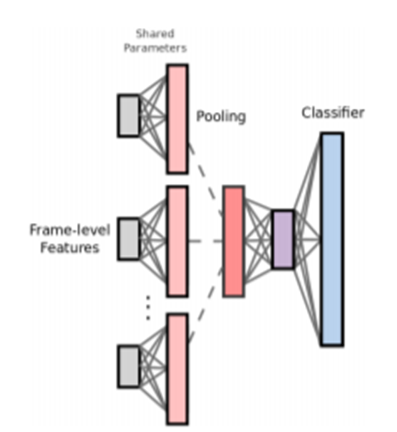
\includegraphics[width=0.4\textwidth]{chapter2/images/DBoF.png}
					\caption{โครงสร้างโมเดลปัญญาประดิษฐ์ของ deep bag of frames}
					\label{fig:dbof}
				\end{figure}
				\item Long short-term memory (LSTM)\\
				โมเดล LSTM ที่ใช้ในบทความนี้นั้นมีการอ้างอิงโครงสร้างมาจากบทความ "Beyond Short Snippets: Deep Networks for Video Classification"\textsuperscript{\cite{yue2015beyond}}
				ซึ่งมีโครงสร้างดังรูปที่ \ref{fig:lstm_full}
				\begin{figure}[!ht]
					\centering
					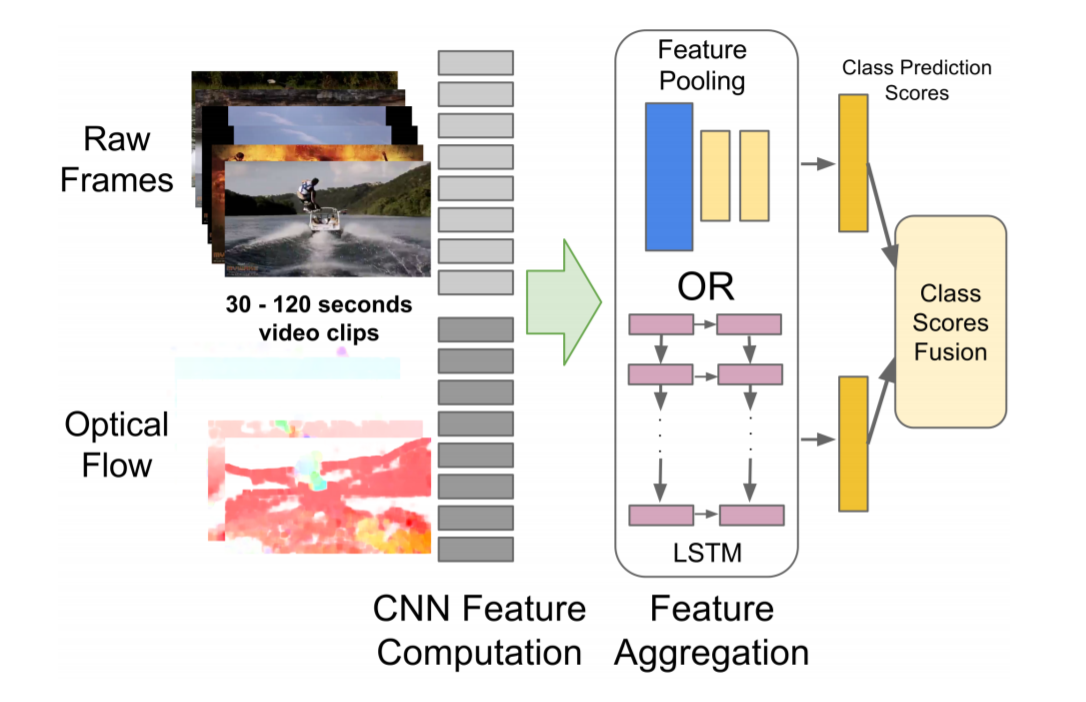
\includegraphics[width=0.6\textwidth]{chapter2/images/lstm_full.png}
					\caption{โครงสร้าง LSTM ที่ใช้การอ้างอิงในบทความนี้}
					\label{fig:lstm_full}
				\end{figure}

				แต่เนื่องจากข้อมูลของ YouTube-8M นั้นไม่สามารถเข้าถึงเฟรมวิดีโอดิบ (raw frame) ได้จึงทำให้สามารถใช้ได้เพียงชั้นของ LSTM และ softmax เท่านั้น
				ซึ่งจากผลการทดลองพบว่า การใช้ LSTM 2 ชั้นที่มี hidden unit 1024 หน่วย นั้นมีประสิทธิภาพมากที่สุด
			\end{enumerate}
		\item โมเดลปัญญาประดิษฐ์ที่ใช้ในการทดสอบชุดข้อมูลแบบที่เป็นคุณลักษณะระดับวิดีโอ
			\begin{enumerate}
				\setlength\itemsep{-0.25em}
				\item Logistic regression\\
				สร้างโมเดลปัญญาประดิษฐ์ของทุกคำกำกับแยกกัน จะได้โมเดลปัญญาประดิษฐ์ 4800 โมเดล โดยที่พารามิเตอร์ $\Theta$ (parameter) ของแต่ละโมเดลหาได้จาก
				\begin{equation}
					\sum_{i=1}^{N}L(y_{i,e}, \sigma(w_eX_i))
				\end{equation}
				\begin{equation}
					L(y_{i,e}, \sigma(w_eX_i)) = y_{i,e}log(\sigma(w_eX_i)) + (1-y_{i,e})log(1-\sigma(w_eX_i))
				\end{equation}
				\begin{equation}
					p(e|X) = \sigma(w_e^TX_i) 
				\end{equation}
				\begin{equation}
					\sigma(z) = \frac{1}{1+exp^{(-z)}}
				\end{equation}
				โดยที่
				\begin{conditions}
					N & จำนวนวิดีโอทั้งหมด\\
					X & คุณลักษณะระดับวิดีโอ\\
					y_{i,e} & คำตอบของคำกำกับ e ในวิดีโอที่ i\\
					w_e & weight ของคำกำกับ e\\
					p(e|X) & ความน่าจะเป็นของคำกำกับ e ของคุณลักษณะระดับวิดีโอ X
				\end{conditions}
				\item Support vector machine (SVM)
				สร้างโมเดลปัญญาประดิษฐ์ของทุกคำกำกับแยกกัน ทำให้จะได้โมเดล SVM 4800 โมเดล โดยได้ใช้ค่า -1 ถึง 1 ในการแสดงถึงคำกำกับด้านลบ (negative label) และคำกำกับค้านบวก (positive label) ตามลำดับ
				และใช้ hinge loss ในการคำนวณหา loss (L) ซึ่งสมการจะเป็นดังนี้
				\begin{equation}
					L(y,\widehat{y}) = max(0,b-(2y-1)\widehat{y}))
				\end{equation}
				โดยที่
				\begin{conditions}
					y & คำตอบจริงของการทำนาย โดยสามารถเป็น 0 หรือ 1 เท่านั้น\\
					\widehat{y} & คำผลการทำนายโดยจะมีค่าอยู่ในช่วง -1 ถึง 1\\
					b & Hinge-loss พารามิเตอร์
				\end{conditions}
				\item Mixture of Expert (MoE)
				Mixture of experts ที่ถูกนำมาใช้ในการอ้างอิงในบทความนี้นั้นมาจากบทความ "Hierarchical mixtures of experts and the EM algorithm"\textsuperscript{\cite{jordan1994hierarchical}}
				โดยการทำนายความน่าจะเป็นว่าคำกำกับ e ในวิดีโอ X ด้วยสมการ 
				\begin{equation}
					p(e|X) = \sum_{h \in H_e} p(h|X)\sigma (u_hX)
				\end{equation}
				ซึ่ง $p(h|X)$ สามารถเขียนได้ในรูปสมการดังนี้
				\begin{equation}
					p(h|X) = \frac{exp(w_hX)}{1+\sum_{h'\in H_e} exp(w_h'X)}
				\end{equation}
				โดยที่
				\begin{conditions}
					H_e & hidden state หรือ expert ของโมเดล\\
					X & วิดีโอที่ใช้ในการทำนายผล\\
					u_h & logistic weight ของ expert $h$\\
					w_h & softmax weight ของ expert $h$\\
					p(h|X) & $|H_e| + 1$ ที่ผ่าน softmax function
				\end{conditions}
				ให้ชุดข้อมูลสำหรับใช้ในการสร้างโมเดล $(x_i, g_i)_{i=1...N} $ โดยที่ $x_i$ คือเวกเตอร์คุณลักษณะ $g_i$ คือคำตอบจริงของการทำนายซึ่งสามารถเป็นได้เพียง 0 และ 1 เท่านั้น 
				และ N คือจำนวนวิดีโอสูงสุด ซึ่งสมการ log-loss ระหว่างผลการทำนายกับคำตอบจริงของการทำนายคือ
				\begin{equation}
					L(p,g)=-glogp-(1-g)log(1-p)
				\end{equation}
				ซึ่งสามารถเขียนในรูปอนุพันธ์ของ softmax weight และ logistic weight ได้ดังนี้
				\begin{equation}
					\frac{\partial L[p_{y|x,g}]}{\partial w_h} = x \frac{p_{h|x}(p_{y|h,x}-p_{y|x})(P_{y|x}-g)}{p_{y|x}(1-p_{y|x})}
				\end{equation}
				\begin{equation}
					\frac{\partial L[p_{y|x,g}]}{\partial u_h} = x \frac{p_{h|x}p_{y|h,x}(1-p_{y|x})(P_{y|x}-g)}{p_{y|x}(1-p_{y|x})}
				\end{equation}
				โดยที่
				\begin{conditions}
					L & log-loss\\
					p & ผลลัพธ์การทำนาย\\
					g & คำตอบจริงของการทำนาย\\
					u_h & logistic weight ของ expert $h$\\
					w_h & softmax weight ของ expert $h$\\
					X & วิดีโอที่ใช้ในการทำนายผล
				\end{conditions}
			\end{enumerate}
		\item เครื่องมือที่ใช้วัดผลสำหรับงานวิจัยนี้ คือ
			\begin{enumerate}
				\setlength\itemsep{-0.25em}
				\item Mean Average Precision (mAP)
				ในแต่ละคำกำกับได้ทำการปัดคะแนนให้อยู่ในช่วง $10^{-4}$ แล้วเรียงลำดับคะแนนทั้งหมดที่ไม่ใช่ 0 จากนั้นให้ค่า $\tau$ เป็นค่าแบ่งเกณฑ์ (threshold)
				โดยที่มี $P(\tau)$ คือ precision และ $R(\tau)$ คือ recall ซึ่งหาได้จาก
				\begin{equation}
					P(\tau) = \frac{\sum_{t \in T}\mathbb{I}(y_t\geq \tau )g_t}{\sum_{t \in T}\mathbb{I}(y_t\geq \tau )}
				\end{equation}
				\begin{equation}
					R(\tau) = \frac{\sum_{t \in T}\mathbb{I}(y_t\geq \tau )g_t}{\sum_{t \in T}g_t}
				\end{equation}
				โดยที่
				\begin{conditions}
					y_t & ค่าความน่าจะเป็นในการทำนาย ซึ่งมีค่าอยู่ในช่วง 0 ถึง 1 \\
					g_t & คำตอบจริงของการทำนาย โดยจะมีค่าเป็นได้แค่ 0 และ 1 เท่านั้น\\
					\mathbb{I}(y_t\geq \tau) & ฟังก์ชั่นซึ่งจะมีค่าเป็น 1 ถ้าหาก $y_t$ มีค่ามากกว่า $\tau$ นอกเหนือจากนั้นจะมีค่าเป็น 0
				\end{conditions}
				สามารถหา average precision ได้จากสมการนี้ 
				\begin{equation}
					AP = \sum_{j=1}^{10000}P(\tau_j)[R(\tau_j)-R(\tau_j+1)]
				\end{equation}
				โดยที่ $\tau = \frac{j}{10000}$
				\clearpage
				\item Hit@k\\
				เหมือนกันกับ Top@k คือการจัดลำดับความน่าจะเป็นของแต่ละคำกำกับจำนวน k อันดับแรก ถ้าหากมีคำกำกับที่ถูกต้องอยู่ในลำดับเหล่านั้น จะถือว่าการทำนายถูกต้อง 
				ซึ่งสามารถเขียนเป็นสมการได้ดังนี้
				\begin{equation}
					\frac{1}{|V|}\sum_{v\in V}V_{e\in G_v}\mathbb{I}(rank_{v,e} \leq k)
				\end{equation}
				โดยที่
				\begin{conditions}
					V & วิดีโอที่ใช้ในการทดสอบทั้งหมด\\
					G_v & คำตอบของวิดีโอ v\\
					rank_{v,e} & อันดับของคำตอบที่ถูกต้อง e ของวิดีโอ v ที่ได้จากการทำนาย\\
					k & อันดับที่ใช้เป็นเกณฑ์
				\end{conditions}
				\item Precision at equal recall rate (PERR)\\
				สำหรับแต่ละวิดีโอจะดูความแม่นยำของผลการทำนาย k อันดับแรก โดยที่ k คือจำนวนคำตอบทั้งหมดของวิดีโอนั้น จากนั้นเฉลี่ยค่าเหล่านั้นด้วยจำนวนวิดีโอทั้งหมด
				สามารถเขียนได้ในรูปสมการดังนี้ โดยใช้ตัวแปรเดียวกันกับของ Hit@k
				\begin{equation}
					\frac{1}{|V :|G_v|>0|}\sum_{v\in V:|G_v|>0}\left [\frac{1}{|G_v|}\sum_{e\in G_v}\mathbb{I}(rank_{v,e} \leq |G_v|) \right ]
				\end{equation}
			\end{enumerate}
		\item ประสิทธิภาพของโมเดลปัญญาประดิษฐ์ที่ใช้ชุดข้อมูลของ YouTube-8M ในการสร้างเทียบกับชุดข้อมูลสำหรับทดสอบของ YouTube-8M
			\begin{table}[!ht]
				\centering
				\begin{tabular}{|c|c|c|c|c|}
					\hline
					{Input features} & {Modeling approach} & {mAP} & Hit@1 & PERR\\
					\hline
					\multirow{3}{*}{Frame-level} & Logistic + average & 11.0 & 50.8 & 42.2\\
					& Deep bag of frames & 26.9 & 62.7 & 55.1\\
					& LSTM & 26.6 & \textbf{64.5} & \textbf{57.3}\\
					\hline
					\multirow{3}{*}{Video-level} & SVM & 17.0 & 56.3 & 47.9\\
					& Logistic regression & 28.1 & 60.5 & 53.0\\
					& Mixture-of-2-experts & \textbf{30.0} & 63.3 & 55.8\\
					\hline
				\end{tabular}
				\caption{ผลการทดสอบโมเดลต่างๆบนชุดข้อมูลสำหรับทดสอบของ YouTube-8M}
				\label{tab: youtube_youtube}
			\end{table}
			\clearpage
		\item โมเดลปัญญาประดิษฐ์ที่ใช้ชุดข้อมูลของ YouTube-8M ในการสร้างแล้วปรับโมเดลด้วยชุดข้อมูลของ Sports-1M เมื่อนำไปทดสอบกับชุดข้อมูลของ Sports-1M 
		พบว่าประสิทธิภาพเมื่อทดสอบด้วย Hit@1 และ Hit@5 สูงสุดอยู่ที่ 65.7\% และ 86.2\% ตามลำดับ ซึ่งใกล้เคียงกับสถิติสูงสุดในตอนนั้นที่ทำไว้ 73.0\% และ 91.0\% (พ.ศ. 2559) 
		โดยที่ใช้เพียงคุณลักษณะจากการเตรียมข้อมูลไว้แล้ว เมื่อเทียบกับสถิติเก่าที่มีการใช้ optical flow เข้ามาช่วย จึงเป็นการพิสูจน์ให้เห็นว่าจำนวนข้อมูลนั้นมีผลต่อการพัฒนาโมเดลปัญญาประดิษฐ์
			
		\item โมเดลปัญญาประดิษฐ์ที่ใช้ชุดข้อมูลของ YouTube-8M ในการสร้างแล้วปรับโมเดลด้วยชุดข้อมูลของ ActivityNet\textsuperscript{\cite{caba2015activitynet}} เมื่อนำไปทดสอบกับชุดข้อมูลของ ActivityNet 
		พบว่าประสิทธิภาพเมื่อทดสอบด้วย mAP สูงสุดอยู่ที่ 77.6\% ในขณะที่สถิติเดิมทำไว้เพียง 53.8\% เป็นการพิสูจน์ว่าชุดข้อมูลนี้นั้นมีความครอบคลุม (generalize) 
		พอที่จะนำไปใช้กับงานประเภทนี้ในหมวดอื่นๆ เนื่องจากว่าจำนวนข้อมูลที่มีขนาดใหญ่และมีความหลากหลาย
		
		\item ปัญหาที่พบ\\
		เนื่องจากว่า YouTube-8M นั้นมีจำนวนข้อมูลที่เยอะมาก ทำให้ไม่สามารถตรวจสอบความถูกต้องของชุดข้อมูลได้ทั้งหมดว่ามีความถูกต้องมากน้อยขนาดไหน 
		ทำให้อาจเกิดข้อผิดพลาดได้ (ปัจจุบันปี 2019 YouTube-8M ได้มีการตรวจสอบข้อมูลอีกครั้ง เพื่อเพิ่มประสิทธิภาพของชุดข้อมูลซึ่งทำให้ปัจจุบันจำนวนข้อมูล 
		และจำนวนคำกำกับลดน้อยลงจากข้อมูลที่ใช้อ้างอิงในบทความข้างต้นที่ได้กล่าวมา)
	\end{enumerate}	
\end{enumerate}